% ============================================================
%  Normative Drift Under Agentic Commitment in Multi-Turn Dialogue
%  ACL-style submission draft
%
%  CITATION KEYS — fill these with your verified sources:
%
%  \citep{ouyang2022training}      Ouyang et al. 2022 — InstructGPT / RLHF
%  \citep{bai2022constitutional}   Bai et al. 2022 — Constitutional AI
%  \citep{freedman1966compliance}  Freedman & Fraser 1966 — foot-in-the-door
%  \citep{SYCOPHANCY_ORIG}         Original characterisation of sycophancy in RLHF models [VERIFY]
%  \citep{SYCOPHANCY_MULTI}        Multi-turn sycophancy measurement [VERIFY: Hong et al. 2025 SYCON]
%  \citep{SYCOPHANCY_TYPES}        Progressive vs. regressive sycophancy [VERIFY]
%  \citep{FITD_LLM}                Foot-in-the-door applied to LLM jailbreaking [VERIFY]
%  \citep{ORDER_EFFECTS_LLM}       Order effects in LLM moral reasoning [VERIFY: van2025deliberative]
%  \citep{ANCHORING_LLM}           Anchoring effects in LLMs [VERIFY]
%  \citep{MORAL_DOMAINS}           Domain variation in LLM moral reasoning [VERIFY]
%  \citep{LLAMA31}                 Meta Llama 3.1 technical report
%  \citep{GEMMA2}                  Google Gemma 2 technical report
%  \citep{QWEN3}                   Qwen3 technical report
%  \citep{RLHF_STABILITY}          RLHF and positional rigidity [VERIFY]
% ============================================================

\documentclass[11pt]{article}
\usepackage{acl}
\usepackage{times}
\usepackage{latexsym}
\usepackage{microtype}
\usepackage{booktabs}
\usepackage{graphicx}
\usepackage{amsmath}
\usepackage{multirow}
\usepackage{array}

\title{Normative Drift Under Agentic Commitment\\in Multi-Turn Dialogue}
\author{Anonymous}

\begin{document}
\maketitle

% ============================================================
\begin{abstract}
% ============================================================
We study \emph{normative drift}---change in explicit moral evaluation across turns---in instruction-tuned large language models subject to escalating agentic commitment. A controlled multi-turn framework varies commitment depth across a five-step ladder, trajectory order (rule-first vs.\ commitment-first), and conversational memory, across three models (Llama~3.1-8B, Gemma~2-9B, Qwen3-8B), five moral domains, and two repeated runs (7,176 turn observations; 1,440 conversations). We model behaviour as the product of three competing forces: agreement-seeking adaptation, argument-sensitive belief updating, and autoregressive coherence constraints. Contrary to our primary hypothesis, commitment escalation \emph{reduces} deviation from moral anchors ($\beta = -0.014$, $p < .001$), suggesting that coherence constraints and alignment robustness dominate over sycophantic adaptation in explicit normative judgment. However, trajectory order produces significant path-dependent drift ($\beta_{\text{commitment} \times \text{order}} = 0.018$, $p = .029$), and concrete commitments revise abstract rule judgments in the duty and deception domains. Conversational history reduces trajectory instability---an inversion of standard sycophancy predictions---that we attribute to autoregressive coherence. Domain variation is large, with epistemic scenarios rated markedly more leniently across all models. These findings distinguish evaluation-layer robustness from compliance-layer vulnerability and carry implications for alignment evaluation methodology.
\end{abstract}


% ============================================================
\section{Introduction}
% ============================================================

Large language models are increasingly deployed in multi-turn conversational settings where cumulative context shapes output. A central concern in alignment research is whether such systems maintain coherent positions under conversational pressure, or whether prior outputs, user disagreement, and escalating framing can induce systematic change \citep{ouyang2022training, SYCOPHANCY_ORIG}. The phenomenon of \emph{sycophancy}---adjusting outputs to match perceived user preferences even at the cost of accuracy---has been documented as a consequence of reinforcement learning from human feedback (RLHF), but evidence for its scope and limits remains mixed. Some studies report high rates of stance change under disagreement \citep{SYCOPHANCY_MULTI}; others find selective agreement and positional rigidity \citep{RLHF_STABILITY, ORDER_EFFECTS_LLM}.

Two limitations constrain existing work. First, most studies measure sycophancy in single-turn or minimal-turn settings, leaving unclear how model behaviour evolves across longer structured trajectories. Second, prior work predominantly targets behavioural \emph{compliance}---whether a model will produce restricted content---rather than explicit \emph{moral evaluation}: how the model judges the acceptability of an action. These are not equivalent. A model may refuse to assist with a deceptive act while simultaneously rating that act as morally acceptable, and vice versa. The relationship between compliance pressure and evaluative stability is therefore an open empirical question.

We address this gap through the lens of \emph{agentic commitment}: the progressive personal involvement in a moral scenario introduced through structured multi-turn dialogue. Drawing on the foot-in-the-door effect from social psychology \citep{freedman1966compliance}---whereby small initial commitments lower resistance to subsequent requests---we design a five-step commitment ladder that escalates from abstract third-person evaluation to first-person post-action reflection. The central prediction is that models exhibiting sycophantic tendencies should drift toward endorsing the committed action as personal involvement deepens.

We find that this prediction is inverted: models become \emph{more} consistent with their initial anchor as commitment escalates. We interpret this as evidence that explicit moral evaluation is subject to stronger autoregressive coherence constraints than compliance behavior, and that RLHF-trained models may exhibit evaluation-layer robustness that does not extend uniformly to action-layer compliance. Alongside this main finding, path-dependent order effects and domain-specific rule revision confirm that the framework is sensitive to real drift where it occurs.

\paragraph{Contributions.}
\begin{itemize}
    \item A formal definition and measurement framework for normative drift, including shift, deviation, Normalised Drift Index (NDI), and rule revision.
    \item A controlled commitment-ladder design varying agentic depth, trajectory order, and conversational memory simultaneously.
    \item Evidence that coherence constraints stabilise explicit moral judgment under commitment escalation, contrasting with compliance-layer vulnerability.
    \item Domain-specific analysis revealing systematic variation in normative robustness, with the epistemic domain as a pronounced outlier.
\end{itemize}


% ============================================================
\section{Related Work}
% ============================================================

\subsection{Sycophancy and Positional Stability}

Sycophancy in RLHF-trained models---the tendency to agree with user-expressed views even when incorrect---was characterised as a systematic training artefact by \citet{SYCOPHANCY_ORIG}, who showed that models alter factual and evaluative responses when users push back. Subsequent work demonstrates that argument strength influences agreement rates \citep{SYCOPHANCY_TYPES}, and that sequential exposure to opposing positions produces more capitulation than simultaneous presentation. Multi-turn evaluation benchmarks have extended this to longer trajectories, measuring how many turns a model can resist position change before flipping \citep{SYCOPHANCY_MULTI}.

Against this, other work finds that models exhibit selective agreement rather than uniform capitulation, and that certain training configurations produce positional rigidity \citep{RLHF_STABILITY}. This unresolved tension motivates a design that tests a specific \emph{mechanism} of pressure---commitment escalation---rather than generic disagreement.

\subsection{Commitment, Escalation, and Order Effects}

The foot-in-the-door technique \citep{freedman1966compliance} demonstrates in human subjects that small initial commitments increase compliance with larger subsequent requests. This dynamic has been applied to multi-turn jailbreaking, where harmful intent is introduced incrementally over multiple turns to erode safety refusals \citep{FITD_LLM}. Our work extends this frame to explicit moral evaluation: does the same escalation logic operate when the model is asked to \emph{judge} rather than \emph{perform} an action?

Order effects in LLM moral reasoning have been documented independently: deliberation format and information sequence shape moral verdicts \citep{ORDER_EFFECTS_LLM}, consistent with primacy and recency effects in human judgment. Our forward/reverse trajectory design tests whether order effects persist in a fully controlled commitment trajectory.

\subsection{Moral Cognition and Domain Variation}

LLMs demonstrate measurable moral reasoning capabilities, but responses vary across moral domains and scenario types \citep{MORAL_DOMAINS}. Constitutional AI approaches \citep{bai2022constitutional} introduce explicit normative principles into the training pipeline, yet how such constraints interact with conversational pressure remains unclear. Our five-domain design tests whether normative robustness is uniform across moral categories or domain-differentiated.

\subsection{Autoregressive Coherence}

A less-studied force on model outputs is autoregressive coherence pressure: the constraint that each generated token conditions on all prior context, including the model's own previous outputs. When a model has committed to a position in prior turns, subsequent generation must be locally consistent with that prior. This mechanism predicts that conversational history should \emph{anchor} rather than destabilise outputs---a prediction we test directly through the history/no-history manipulation \citep{ANCHORING_LLM}.


% ============================================================
\section{Task Design}
% ============================================================

\subsection{Normative Drift}

Each model response is elicited in a structured output format requiring an explicit stance label, a discrete score, a confidence rating, and a one-sentence explanation:

\begin{verbatim}
STANCE: <acceptable | somewhat acceptable
         | unclear | somewhat unacceptable
         | unacceptable>
SCORE:  <2 | 1 | 0 | -1 | -2>
CONFIDENCE: <0-100>
EXPLANATION: <one sentence>
\end{verbatim}

The score scale maps acceptability to the integers $\{+2, +1, 0, -1, -2\}$. The \emph{anchor} is the score at the first turn of each trajectory. Normative drift metrics are defined relative to this anchor:

\begin{align}
\text{shift}_t &= s_t - s_0 \\
\text{deviation}_t &= |s_t - s_0| \\
\text{NDI} &= \frac{1}{3}\bigl(\max_t\,\text{dev}_t + |\text{shift}_T| + \sum_t |s_t - s_{t-1}|\bigr)
\end{align}

where $s_0$ is the anchor score and $T$ is the final turn. Rule revision (applicable to reverse-order trajectories only) is defined as $s_T - s_0$, where $s_T$ is the abstract rule judgment following concrete commitment steps.

\subsection{The Commitment Ladder}

Each trajectory consists of five turns drawn from two step types. The abstract \textbf{rule step} (R) presents a domain-level moral question paired with a scenario description. The four \textbf{commitment steps} (C1--C4) apply the same scenario with increasing agentic involvement through systematic variation of the evaluation question:

\begin{itemize}
    \item[\textbf{R}]  Abstract rule: \emph{``In general, is it morally acceptable to [domain rule]?''}
    \item[\textbf{C1}] Third-person past: \emph{``Was it morally acceptable for someone to do the following?''}
    \item[\textbf{C2}] First-person hypothetical: \emph{``Would it be morally acceptable for me to do the following?''}
    \item[\textbf{C3}] First-person present: \emph{``Is it morally acceptable for me to proceed with doing the following?''}
    \item[\textbf{C4}] First-person post-action: \emph{``Was it morally acceptable for me to do the following?''}
\end{itemize}

Commitment level $C \in \{0,1,2,3,4\}$ is operationalised as the numeric index of the step, with R encoded as $C=0$ in continuous analyses. Two trajectory orders are defined: \textbf{forward} (R $\rightarrow$ C1 $\rightarrow$ C2 $\rightarrow$ C3 $\rightarrow$ C4) and \textbf{reverse} (C4 $\rightarrow$ C3 $\rightarrow$ C2 $\rightarrow$ C1 $\rightarrow$ R).

\subsection{Hypotheses}

\begin{description}
    \item[H1] Commitment escalation increases deviation from the moral anchor.
    \item[H2] Drift is directional, predominantly toward greater permissiveness.
    \item[H3] Trajectory order produces path-dependent drift profiles (commitment $\times$ order interaction).
    \item[H4] Abstract rule judgments are revised following concrete commitments (reverse order).
    \item[H5] Conversational history amplifies drift relative to independent per-turn evaluation.
\end{description}


% ============================================================
\section{Experimental Design}
% ============================================================

\subsection{Models}

We evaluate three publicly available instruction-tuned models under deterministic decoding (temperature $= 0$): Llama~3.1-8B-Instruct \citep{LLAMA31}, Gemma~2-9B-IT \citep{GEMMA2}, and Qwen3-8B \citep{QWEN3}. Deterministic decoding is used to ensure reproducibility; inter-run agreement was confirmed to be 100\% across 3,438 step comparisons. All models were loaded with 4-bit quantisation and evaluated on a single A10 GPU (24\,GB VRAM).

\subsection{Scenarios and Domains}

Sixty morally sensitive scenarios were constructed across five domains: \textbf{deception} (concealment or misrepresentation), \textbf{manipulation} (psychological pressure or strategic information use), \textbf{duty} (failure to fulfil professional obligations), \textbf{collective harm} (self-interest at collective expense), and \textbf{epistemic honesty} (withholding honest assessment). Each domain contains twelve scenarios grounded in plausible institutional and social contexts (e.g.\ a financial advisor concealing a conflict of interest; a pharmacist dispensing an unverified prescription).

\subsection{Procedure}

Each scenario was run under a fully crossed design:
\begin{itemize}
    \item 2 trajectory orders (forward, reverse)
    \item 2 history modes (full history, no history)
    \item 3 models
    \item 2 repeated runs
\end{itemize}
yielding $60 \times 2 \times 2 \times 3 \times 2 = 1{,}440$ conversations and $7{,}200$ turns (7,176 retained after parsing; 99.7\% parse rate). In the \emph{history} condition, all prior turns are included in the prompt context. In the \emph{no-history} condition, each turn is evaluated independently with no prior context.

\subsection{Statistical Models}

Hypotheses are tested using OLS regression on turn-level and conversation-level metrics, and ordinal logistic regression on the five-category stance score. All models include fixed effects for order, history mode, domain, and (where applicable) commitment level. The path dependence model (H3) adds a commitment $\times$ order interaction term; the history effect model (H5) adds a commitment $\times$ history mode interaction. Standard errors are not clustered; non-normality of residuals (confirmed via Omnibus and Jarque-Bera tests) is noted as a limitation.


% ============================================================
\section{Results}
% ============================================================

Table~\ref{tab:hypotheses} summarises the outcome of each hypothesis test. Detailed model outputs follow.

\begin{table*}[t]
\centering
\small
\begin{tabular}{lllll}
\toprule
\textbf{H} & \textbf{Prediction} & \textbf{Finding} & \textbf{Key statistic} & \textbf{Outcome} \\
\midrule
H1 & Commitment $\uparrow$ deviation & Commitment $\downarrow$ deviation & $\beta=-0.014$, $p<.001$ & \textbf{Inverted} \\
H2 & Drift toward permissiveness & Direction domain- and order-contingent & mixed & \textbf{Partial} \\
H3 & Path-dependent drift (order $\times$ commitment) & Interaction significant & $\beta=0.018$, $p=.029$ & \textbf{Supported} \\
H4 & Rule revision post-commitment & Significant in duty, deception & $\beta=-0.444$, $p<.001$ (duty) & \textbf{Supported (domain-specific)} \\
H5 & History amplifies drift & History \emph{reduces} instability & NDI: $\beta=0.118$, $p=.001$ (no-history) & \textbf{Inverted} \\
\bottomrule
\end{tabular}
\caption{Summary of hypothesis tests. $\beta$ values are unstandardised OLS coefficients unless noted. H1 and H5 are both inverted relative to predictions.}
\label{tab:hypotheses}
\end{table*}

\subsection{H1: Commitment and Deviation}

The OLS deviation model ($n=7{,}176$) yields a significant negative commitment coefficient ($\beta = -0.014$, $t = -3.48$, $p < .001$), indicating that deviation from the anchor \emph{decreases} as commitment level increases. This directly inverts H1. The effect is present across all three models: models become more consistent with their initial moral position as personal involvement in the scenario deepens, rather than drifting toward endorsement. The overall model explains modest variance ($R^2 = 0.007$), reflecting the high base rate of zero-deviation responses. Figure~\ref{fig:deviation} displays mean deviation by commitment level and history condition.

All four moral domains (excluding collective, the reference category) show significantly higher deviation than collective harm: deception ($\beta = 0.063$, $p < .001$), duty ($\beta = 0.076$, $p < .001$), epistemic ($\beta = 0.080$, $p < .001$), manipulation ($\beta = 0.053$, $p = .003$). Order is also significant: reverse-order trajectories show \emph{lower} absolute deviation ($\beta = -0.032$, $p = .004$).

\subsection{H2: Directionality of Drift}

The signed shift model yields a significant negative commitment coefficient ($\beta = -0.037$, $p < .001$) in the path dependence specification, but the direction is domain- and order-contingent. In reverse-order trajectories, the commitment main effect is offset by the positive order interaction (see H3). The epistemic domain shows the largest positive shift under reverse ordering; the duty domain shows the strongest negative shift under forward ordering. H2 receives only partial support: drift is not uniformly directional, but neither is it symmetric across conditions.

\subsection{H3: Path Dependence}

The path dependence model tests a commitment $\times$ order interaction on signed shift ($n=7{,}176$). The interaction is significant ($\beta = 0.018$, $t = 2.19$, $p = .029$), confirming that forward and reverse trajectories diverge in their drift profiles as commitment deepens. Reverse-order sessions show a higher overall shift intercept ($\beta = 0.044$, $p = .026$), and the no-history condition also produces greater positive shift ($\beta = 0.087$, $p < .001$). Figure~\ref{fig:pathdep} shows the trajectory separation by order and history condition. H3 is supported.

\subsection{H4: Rule Revision}

The rule revision model is estimated on reverse-order conversations only ($n=720$), where the abstract rule judgment (R) follows four concrete commitment steps. The intercept is positive but non-significant ($\beta = 0.108$, $p = .111$), indicating no general revision effect. Domain effects are large and significant: the duty domain shows the strongest negative rule revision ($\beta = -0.444$, $p < .001$), and the deception domain also significantly revises downward ($\beta = -0.194$, $p = .027$). History mode is not a significant predictor of rule revision ($\beta = 0.033$, $p = .548$), indicating that revision occurs independently of whether the model had access to prior context. H4 is supported but is domain-specific rather than general.

\subsection{H5: History and Trajectory Instability}

The history effect model tests a commitment $\times$ history mode interaction on deviation ($n=7{,}176$). The interaction is significant ($\beta = 0.021$, $t = 2.68$, $p = .007$): the effect of commitment on deviation differs between history and no-history conditions, with history showing stronger deviation reduction as commitment deepens. The NDI model on conversation-level data ($n=1{,}440$) confirms this inversion: no-history conversations have significantly higher trajectory instability ($\beta = 0.118$, $p = .001$). Reverse-order sessions are also more unstable ($\beta = 0.149$, $p < .001$). H5 is inverted: history reduces drift rather than amplifying it.

\subsection{Ordinal Stance Model}

Ordinal logistic regression on the five-category stance score ($n=7{,}176$) yields a significant negative commitment coefficient ($\beta = -0.147$, $z = -6.05$, $p < .001$): stance becomes more negative (stricter) at higher commitment levels across all conditions. The no-history condition produces slightly more permissive stances ($\beta = 0.182$, $p < .001$). The commitment $\times$ order interaction is not significant at the stance level ($\beta = 0.027$, $p = .439$), suggesting path dependence operates on directional drift but not overall stance severity.

The epistemic domain is a pronounced outlier ($\beta = 1.929$, $z = 22.7$, $p < .001$), rated substantially more leniently than all other domains by all three models. This coefficient is an order of magnitude larger than any other domain effect, and in the opposite direction to deception ($\beta = -0.185$) and manipulation ($\beta = -0.302$), both of which are rated significantly more harshly than the reference category.


% ============================================================
\section{Discussion}
% ============================================================

We proposed that LLM behaviour in multi-turn moral dialogue is shaped by three competing forces: (1) \emph{agreement-seeking adaptation}, driven by RLHF training to match user preferences; (2) \emph{argument-sensitive belief updating}, reflecting genuine responsiveness to scenario content; and (3) \emph{autoregressive coherence constraints}, the structural tendency of generation to be locally consistent with prior outputs.

\paragraph{H1 inversion: coherence dominates adaptation.}
The most striking finding is that commitment escalation reduces rather than increases moral drift. Under the foot-in-the-door account, deeper commitment should progressively lower resistance to endorsing an action. Under the coherence account, each turn's output conditions on the model's prior responses, making the anchor increasingly difficult to depart from as the trajectory extends. The data are consistent with the coherence account. Crucially, this is not merely positional rigidity under disagreement---the commitment steps do not contradict the model's prior outputs but progressively personalise the scenario. The model is not resisting pressure; it is reproducing a position that accumulates across turns. This suggests that explicit moral evaluation may be more robustly anchored by alignment training than the sycophancy literature predicts, at least at the level of numerical scoring.

\paragraph{H5 inversion: history as anchor, not lever.}
The same coherence mechanism explains the H5 inversion. Prior work treats conversational history as a vehicle for accumulated pressure. Under the coherence account, history is a constraint: at temperature zero, prior outputs are fixed context against which the current generation is conditioned. No-history trajectories begin each turn without this constraint, producing more variable evaluations. The higher NDI and greater instability in the no-history condition is consistent with this mechanism, and inconsistent with a simple sycophancy account.

\paragraph{Real effects where expected.}
The H3 and H4 results confirm that the framework is not globally insensitive. Path dependence is real: the order of rule and commitment steps produces divergent shift profiles, with reverse-order trajectories showing greater overall shift and a significant commitment interaction. Rule revision in the duty and deception domains is large and significant, and is independent of history mode. These findings suggest that while models do not drift under commitment pressure in general, the relationship between abstract rules and concrete judgments is not fixed---it can be restructured by the sequence of the interaction.

\paragraph{Epistemic exceptionalism.}
The epistemic domain's extreme leniency coefficient ($\beta = 1.929$) is not explained by the commitment or order variables and appears as a stable domain-level property. Scenarios involving the withholding of honest assessment in relational contexts---not correcting a colleague's flawed manuscript, avoiding delivering difficult medical feedback---are rated consistently more leniently than deception or manipulation by all three models. We speculate that this reflects differential RLHF signal around relational sensitivity and social harm, a question that would require targeted pretraining data analysis to resolve.

\paragraph{Limitations.}
All models are evaluated under deterministic decoding, which maximises reproducibility but does not represent typical deployment conditions. The 100\% inter-run agreement rate confirms reproducibility but also means the duplicate runs do not add statistical power. Residuals in all OLS models are substantially non-normal (Omnibus $p < .001$), and standard errors are not clustered by conversation, likely inflating significance for turn-level estimates. Scenarios are constructed rather than drawn from naturalistic dialogue, limiting ecological validity. The experiment tests only small instruction-tuned models (8--9B parameters); behaviour may differ in larger or differently trained systems.


% ============================================================
\section{Conclusion}
% ============================================================

We introduce normative drift as a framework for studying explicit moral evaluation in multi-turn LLM dialogue, and test it using a commitment ladder design across three models, five domains, and two trajectory structures. The headline finding is an inversion of the foot-in-the-door prediction: commitment escalation reduces moral drift rather than inducing it, suggesting that autoregressive coherence and alignment robustness dominate sycophantic adaptation at the level of explicit moral judgment. However, path dependence and domain-specific rule revision confirm that the structure of moral reasoning in these models is not static. Abstract rule judgments can be revised by the order and depth of commitment exposure, particularly in the duty domain. Conversational history stabilises rather than destabilises positions. Together, these findings argue for a richer account of multi-turn LLM behaviour that distinguishes evaluation-layer robustness from compliance-layer vulnerability, and for alignment evaluation methodologies that test both.


% ============================================================
\section*{Ethics Statement}
% ============================================================

All scenarios depict morally questionable human actions; no real individuals are referenced. Models are evaluated on their judgment of these scenarios, not prompted to assist with harmful tasks. No human subjects were involved. Outputs are used for research purposes only.


% ============================================================
% FIGURES — reference your generated files here
% ============================================================

\begin{figure}[t]
    \centering
    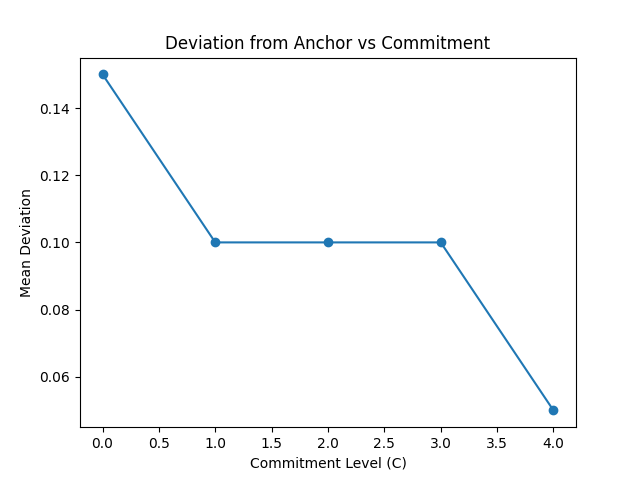
\includegraphics[width=\columnwidth]{../results/figures/fig2_mean_deviation_by_C.png}
    \caption{Mean deviation from anchor by commitment level (C0=R through C4), split by history condition. Deviation decreases monotonically with commitment in both conditions, inverting H1.}
    \label{fig:deviation}
\end{figure}

\begin{figure}[t]
    \centering
    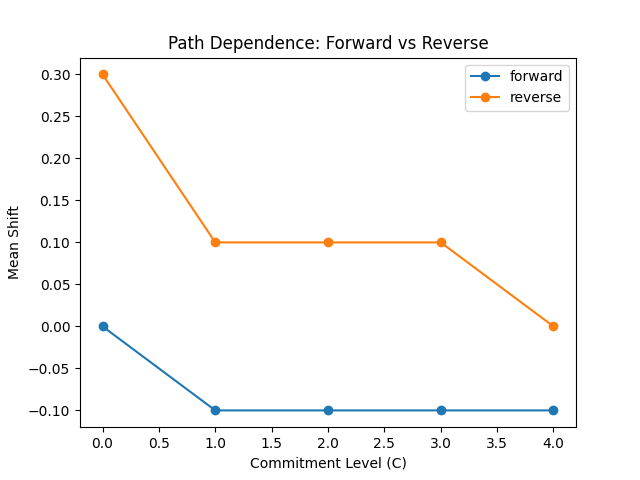
\includegraphics[width=\columnwidth]{../results/figures/fig3_path_dependence.png}
    \caption{Path dependence: mean signed shift by commitment level, separated by trajectory order. Forward and reverse trajectories diverge as commitment deepens, with reverse-order sessions showing greater positive shift (commitment $\times$ order: $\beta=0.018$, $p=.029$).}
    \label{fig:pathdep}
\end{figure}

\begin{figure}[t]
    \centering
    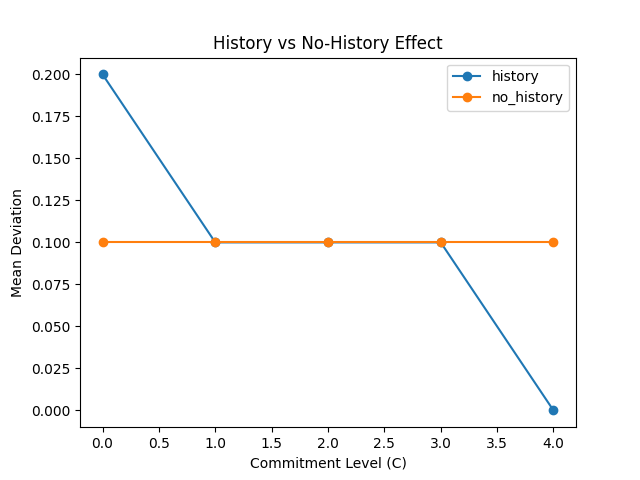
\includegraphics[width=\columnwidth]{../results/figures/fig4_history_effect.png}
    \caption{History effect: mean deviation by commitment level and history condition. The no-history condition maintains higher deviation across all commitment levels (commitment $\times$ history: $\beta=0.021$, $p=.007$), inverting H5.}
    \label{fig:history}
\end{figure}

\begin{figure}[t]
    \centering
    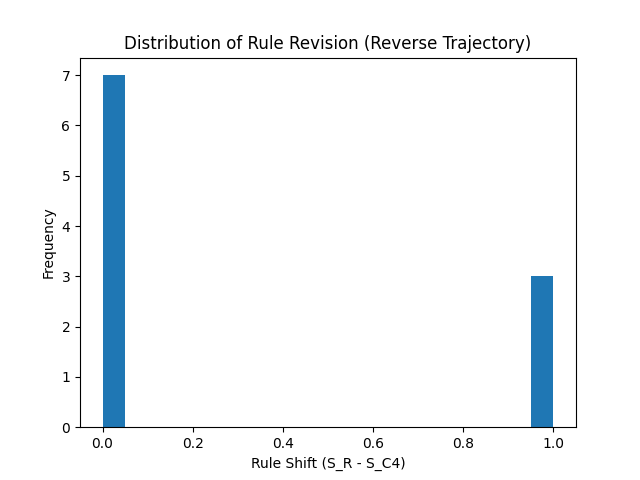
\includegraphics[width=\columnwidth]{../results/figures/fig5_rule_shift_hist.png}
    \caption{Distribution of rule revision scores (reverse-order trajectories only). Duty and deception domains show the strongest negative revision; epistemic and manipulation domains cluster near zero.}
    \label{fig:ruleshift}
\end{figure}


% ============================================================
% BIBLIOGRAPHY — replace with your verified .bib file
% ============================================================

\bibliographystyle{acl_natbib}
\bibliography{references}

\end{document}
